\subsection{Расчет скоростей слабых распадов} \label{sec:weakfit}

  Помимо реакций нейтронного захвата, важную роль в $r$-процессе играют $\beta^-$-распады. Скорость слабых распадов сильно зависит массы распадающегося и конечного ядер, на что указывает хорошо известное соотношение Сарджента $\lambda \sim Q^5$, связывающее скорость распада $\lambda$ с энерговыделением $Q$. Для учета влияния выбора массовой модели на распределение продуктов $r$-процесса следовало бы рассчитывать скорости не только реакции $(n,\gamma)$, но и $\beta$-распадов, варьируя массовую модель. К сожалению, в открытом доступе нами не было обнаружено готовых программ, позволяющих рассчитывать скорости слабых распадов, задавая различные массы исходного и конечного ядер. Собственная же реализация подобной программы представляет из себя отдельную, весьма непростую задачу.

  Отметим, что в условиях астрофизического $r$-процесса по его определению характерные времена $\beta^-$-распадов превышают скорости реакции $(n,\gamma)$ на порядки. Таким образом для достижения удовлетворительной точности симуляции $r$-процесса, в особенности на коротких промежутках времени около $1$~с, достаточно задать скорости слабых распадов приблизительно, с точностью до порядка. В связи с этим нами было решено использовать данные о скоростях $\beta^-$-распадов, представленные в библиотеке REACLIB, не меняя их.

\begin{figure}[b!]
  \centering
  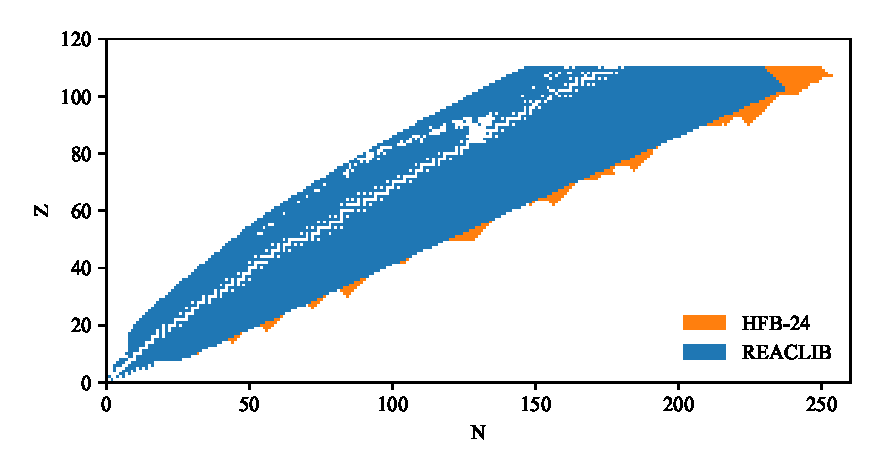
\includegraphics[width=0.8\textwidth]{pics/chart_weak_comparison.eps}
  \caption{Данные о слабых распадах из библиотеки REACLIB (синие квадраты) и нейтроноизбыточные изотопы, присутствующие в таблице масс HFB-24, но отсутствующие в REACLIB (оранжевые квадраты).}
  \label{img:weak_comparison}
\end{figure}

  Возникает, однако, другая проблема. Выбор ядерной массовой модели влияет не только на значения скоростей ядерных реакций, но и на границы существования ядер, определяемые знаком энергий отделения протона $B_p$ и нейтрона $B_n$:
  \begin{equation}\begin{aligned}\label{eq:driplines}
    B_p(A,Z) &= E_{\text{св}}(A,Z) - E_{\text{св}}(A-1,Z-1),\\
    B_n(A,Z) &= E_{\text{св}}(A,Z) - E_{\text{св}}(A-1,Z)
  \end{aligned}\end{equation}
  При отрицательных значениях $B_p$ или $B_n$ протон или нейтрон, соответственно, будет беспрепятственно покидать ядро. Значения энергий связи $E_{\text{св}}$ в выражениях \ref{eq:driplines} определяются предсказаниями ядерных массовых моделей. Ясно, что положение линии отделения нейтрона должно существенно влиять на протекание $r$-процесса, потому что в области $B_n < 0$ накопление нейтронов становится невозможным.

\begin{figure}
  \centering
  %\begin{subfigure}{0.48\textwidth}
  %  \centering
  %  \includegraphics[width=\textwidth]{pics/decay_fit26.eps}
  %  \caption{Железо}
  %\end{subfigure}
  %\hfill
  \begin{subfigure}{0.48\textwidth}
    \centering
    \includegraphics[width=\textwidth]{pics/decay_fit65.eps}
    \caption{Тербий}
  \end{subfigure}
  \hfill
  \begin{subfigure}{0.48\textwidth}
    \centering
    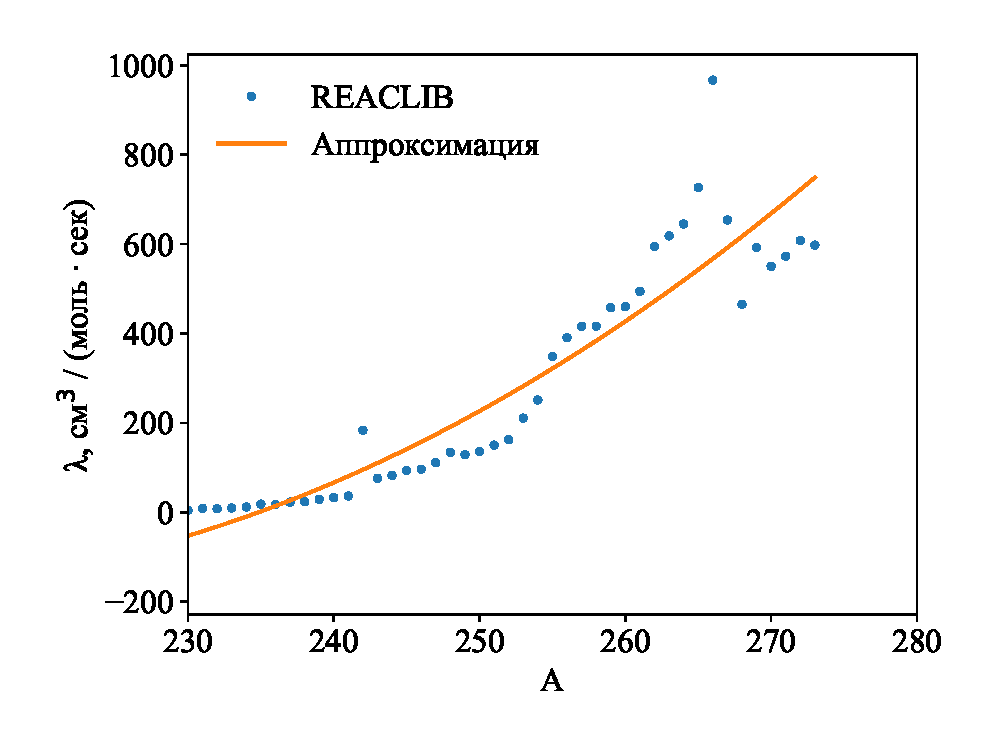
\includegraphics[width=\textwidth]{pics/decay_fit82.eps}
    \caption{Свинец}
  \end{subfigure}
  \caption{Экстраполяция скоростей слабых распадов для нейтроноизбыточных ядер полиномом второй степени на основе данных из библиотеки REACLIB.}
  \label{img:weak_decay_fit}
\end{figure}

  Если ядерная модель предсказывает, что линия отделения нейтронов лежит в пределах массива данных REACLIB, то проблем не возникает. Однако это не всегда так, в чем можно убедиться по рис.~\ref{img:weak_comparison}, показывающему ядра, представленные в HFB-24, но отсутствующие в REACLIB. Отметим, что и в REACLIB, и в различных таблицах теоретических масс ядер дополнительно представлены данные для изотопов вне области существования ядер, находящиеся вблизи границ отделения протона и нейтрона. Эти данные не являются избыточными, так как позволяют учитывать, что под воздействием интенсивных нейтронных захватов ядро все таки может выйти за границу отделения и просуществовать там некоторое время. Как видно по рисунку, область ядер, для которых есть предсказания массовой модели HFB-24, но отсутствуют значения скоростей $\beta^-$-распада, весьма велика. Если не внести в симуляцию $r$-процесса скорости $\beta^-$-распада для этих изотопов, то они будут исчезать только за счет реакции выбивания нейтрона $\gamma$-квантом и могут накапливаться.    

  Как уже было сказано, при моделировании $r$-процесса скорости $\beta^-$-распада достаточно задать приблизительно, воспользовавшись простой экстраполяцией параболой. Нами также рассматривалась более качественная модельная функция, использующая правило Сарджента $\lambda \sim Q^5$, где энерговыделение $Q$ можно было бы связать с массовым числом $A$ через формулу Вайцзеккера для энергии связи. Такая аппроксимация менее удобна из-за большего числа параметров, а существенного выигрыша в точности не дает. Кроме того, следует учесть, что с приближением к границе существования ядер обычный $\beta^-$-распад начинает подавляться слабыми распадами с вылетом двух и трех нейтронов. Учесть это обстоятельство в качественной модельной функции было бы затруднительно. Поэтому в итоге мы остановились на простейшей экстраполяции полиномом второй степени. Результаты экстраполяции скоростей $\beta^-$-распада для нейтроноизбыточных изотопов тербия и свинца представлены на рис.~\ref{img:weak_decay_fit}.

